\section{Group Convolutions}\label{sec:group_convolutions}

The first significant extension of classical \glspl{CNN} emerges upon recognizing that translations represent only a special case of a broader group of geometric transformations. Group convolutions provide a rigorous theoretical framework for incorporating additional symmetries such as rotations, reflections, and more complex transformations, while preserving the equivariance properties that make convolutional architectures powerful.

This section explores how group theory and harmonic analysis provide the mathematical tools needed to design neural architectures that automatically respect the symmetries inherent to different data domains. The foundations of group representation theory are found in the classical works of \citet{Peter1927} and \citet{Serre1977}.

\subsection{Theoretical Foundations}\label{subsec:fundamentos_teoricos}

The group-theoretic foundations needed for group convolutions (groups, group actions, equivariance, homogeneous spaces) are fully developed in \autoref{ch:gdl}, Sections~\ref{subsec:teoria_grupos_representaciones} and~\ref{subsec:equivarianza_invarianza}. This section focuses on the specific application of these concepts to geometric convolutions.

Recall that a function $\Phi$ between function spaces is \textit{$G$-equivariant} (\autoref{def:equivariance_gdl}, \autoref{ch:gdl}) if $\Phi(L_g f) = L_g' (\Phi(f))$ for all $g \in G$, and \textit{$G$-invariant} if $\Phi(L_g f) = \Phi(f)$. Equivariance generalizes the translation invariance of classical \glspl{CNN}: if the data possess symmetries under $G$, $G$-equivariant functions preserve these symmetries throughout processing, resulting in more robust and parameter-efficient representations.

\subsubsection{Convolution on Groups}

The generalization of the convolution operation to arbitrary groups constitutes the theoretical core of the geometric extensions of \glspl{CNN}.

\begin{definition}[Group Convolution]
For functions $f, \psi: G \to \mathbb{R}$ defined over a group $G$, the \textbf{group convolution} is defined as:
\begin{equation}
(f *_G \psi)(u) = \int_G f(uv^{-1}) \psi(v) \, d\mu(v)
\label{eq:group_convolution}
\end{equation}
where $\mu$ is the Haar measure on $G$.
\end{definition}

This definition generalizes the classical convolution by replacing the subtraction operation $u - v$ with the group operation $uv^{-1}$. For discrete groups, the integral becomes a sum.

The following theorem establishes the fundamental connection between equivariance and convolution in the context of neural networks:

\begin{theorem}[Kondor-Trivedi, \citep{kondor2018generalizationconvolutionalneural}]
A feedforward neural network $N$ is equivariant to the action of a compact group $G$ on its inputs if and only if each layer of $N$ implements a generalized form of convolution derived from equation \ref{eq:group_convolution}.
\end{theorem}

\begin{proof}[Sketch of the proof]
The proof is based on two directions:

\textbf{Forward direction:} If each layer implements group convolution, then by construction it preserves the group structure, which implies equivariance.

\textbf{Converse direction:} If the network is equivariant, then via representation-theoretic techniques one can show that the linear transformations between layers must have the form of generalized convolutions.

The complete proof uses harmonic analysis and representation theory to characterize all possible equivariant linear transformations.
\end{proof}

\subsubsection{Representation Theory}

Representation theory provides the mathematical tools to analyze how groups act on vector spaces, which is essential for the design of equivariant architectures. The fundamental concepts of group representations, including irreducible representations and the decomposition theorem, are developed in \autoref{ch:gdl}, Section~\ref{subsec:teoria_grupos_representaciones}.

In summary, a \textit{representation} is a homomorphism $\rho: G \to GL(V)$ that allows one to ``linearize'' the action of the group, and the \textit{irreducible representations} (\autoref{def:representacion_irreducible}) are the fundamental building blocks from which all other representations are constructed.

\subsubsection{Harmonic Analysis on Groups}

Harmonic analysis generalizes concepts such as the Fourier transform to non-abelian groups, providing powerful tools for frequency analysis in more general domains.

The foundations of this harmonic analysis on groups are based on representation theory. The basic concepts of groups, homomorphisms, and Lie groups are established in \autoref{ch:gdl}, Section~\ref{subsec:teoria_grupos_representaciones}, while here we develop the specific aspects of representations in the context of geometric convolutions.

For the complete theory of group representations, including definitions, decomposition theorems, and the Peter-Weyl theorem, see \autoref{ch:gdl}, Section~\ref{subsec:teoria_grupos_representaciones}. Here we focus on its specific application to the harmonic analysis of convolutions.

In the context of equivariant \glspl{CNN}, each layer processes features that transform under specific representations of the symmetry group (\autoref{def:representacion_grupo}, \autoref{ch:gdl}). The choice of these representations (that is, of the homomorphism $\rho: G \to GL(V)$ where $V$ is the feature space) determines what types of patterns the network can detect equivariantly.

\begin{example}[Regular Representation in \glspl{GCNN}]\label{ex:representacion_regular_cnn}
For a finite group $G = \{g_1, g_2, \ldots, g_n\}$, the \textbf{left regular representation} acts on functions $f: G \rightarrow \mathbb{R}^d$ via:
\begin{equation}
(\rho(g)f)(h) = f(g^{-1}h)
\end{equation}
This representation is fundamental in G-\glspl{CNN}, where the channels correspond to evaluations of the function at different group elements.
\end{example}

\textbf{Decomposition of Representations.} By the decomposition theorem (\autoref{thm:descomposicion_representaciones}, \autoref{ch:gdl}), every representation of a compact group decomposes into a direct sum of irreducible representations. In the context of G-\glspl{CNN}, this has direct consequences for architecture design.

\textbf{Implications for CNN Design.} The Peter-Weyl theorem (\autoref{thm:peter_weyl}, \autoref{ch:gdl}) guarantees that $L^2(G) = \bigoplus_{\lambda \in \widehat{G}} n_\lambda \mathcal{H}_\lambda$, where each $\mathcal{H}_\lambda$ is the space of an irreducible representation. This has direct consequences for G-\glspl{CNN}: the decomposition into irreducible representations $\mathcal{H}_\lambda$ determines the optimal channel structure. Each $\mathcal{H}_\lambda$ corresponds to a channel type, and $n_\lambda$ indicates how many channels of that type to include in order to fully capture the symmetries of the group.

\subsubsection{Fourier Analysis on Groups}

The Fourier transform on groups (Equation~\ref{eq:fourier_grupo_finito}) generalizes to the continuous case by replacing the sum with an integral over the Haar measure: $\hat{f}(\rho_i) = \int_G f(g) \rho_i(g) \, d\mu(g)$. The convolution theorem (Equation~\ref{eq:convolucion_fourier_grupos}) extends identically, turning the group convolution into a matrix product of the transforms.

\subsubsection{Homogeneous Spaces}

In practical applications, functions are defined over homogeneous spaces $X = G/H$ where $H$ is a subgroup of $G$, rather than over the full group.

\begin{definition}[Homogeneous Space]
A space $X$ is \textbf{homogeneous} under the action of $G$ if for any $x, y \in X$, there exists $g \in G$ such that $g \cdot x = y$.
\end{definition}

The sphere $S^2$ is homogeneous under $SO(3)$, and regular images are homogeneous under translations. The generalization of convolutions to homogeneous spaces requires additional lifting and projection techniques.

\subsubsection{Connection with Classical CNNs}

Classical \glspl{CNN} are a special case of group convolutions where $G = (\mathbb{Z}^2, +)$ acts by translations on discrete images. In this case:

\begin{itemize}
    \item The irreducible representations are one-dimensional (characters)
    \item The group convolution reduces to the classical convolution
    \item The filters are translation-invariant
\end{itemize}

The geometric extensions incorporate richer groups such as $\gls{SO2}$ for rotations, $SE(2)$ for planar rigid motions, or $\gls{SO}$ for three-dimensional rotations.

\subsubsection{Unified Theoretical Framework}

The theoretical framework presented provides the foundations for developing specific architectures:

\begin{enumerate}
    \item \textbf{Group identification}: Determine which symmetries are present in the data
    \item \textbf{Representation analysis}: Characterize the relevant irreducible representations
    \item \textbf{Convolution design}: Implement equivariant operations efficiently
    \item \textbf{Optimization}: Exploit the group structure to reduce parameters
\end{enumerate}

This theoretical framework establishes the rigorous mathematical foundations on which the various extensions of group convolutions we will explore in the following subsections are built, from finite groups to complex manifolds, always preserving the fundamental principles of equivariance and computational efficiency.

A deep understanding of these theoretical foundations is essential to appreciate both the capabilities and the limitations of each specific extension, as well as for the design of new architectures that exploit particular symmetries present in specific application domains.

\subsection{Equivariant Universality Theorem}\label{subsec:teorema_universalidad_equivariante}

A fundamental result in the theory of group convolutions establishes that equivariant architectures can approximate any continuous equivariant function. This theorem provides theoretical justification for the use of group convolutions and guarantees their expressive power.

\begin{theorem}[Equivariant Universality for CNNs]\label{theorem:equivariant_universality_cnns}
    Let $G$ be a compact group acting on a compact domain $\mathcal{D}$, and let $\mathcal{F}_G$ be the space of continuous $G$-equivariant functions from $L^2(\mathcal{D})$ to $L^2(\mathcal{D})$. For any $f \in \mathcal{F}_G$ and $\epsilon > 0$, there exists a $G$-equivariant convolutional network $\Phi_{\text{G-CNN}}$ such that:
    \begin{equation}
        \|f - \Phi_{\text{G-CNN}}\|_{L^2} < \epsilon
    \end{equation}
    That is, \glspl{GCNN} are universal approximators in the space of equivariant functions.
\end{theorem}

\subsubsection{Constructive Proof for the Discrete Group $\mathbb{Z}^2$}

We present a simplified proof for the case of the discrete translation group $\mathbb{Z}^2$, which illustrates the main ideas of the general theorem.

\textbf{Step 1: Spectral Decomposition}

For a function $f: \mathbb{Z}^2 \to \mathbb{R}$ of compact support, the discrete Fourier transform allows us to write:
\begin{equation}
    f(x) = \sum_{k \in \mathbb{Z}^2} \hat{f}(k) e^{2\pi i \langle k, x \rangle / N}
\end{equation}

\textbf{Step 2: Approximation by Convolutions}

Each frequency component can be approximated by a convolution with an appropriate filter. For frequency $k$, we define:
\begin{equation}
    g_k(x) = \frac{1}{N^2} e^{2\pi i \langle k, x \rangle / N}
\end{equation}

\textbf{Step 3: Construction of the Network}

A convolutional network with $M$ filters in the first layer can be expressed as:
\begin{equation}
    \Phi_{\text{CNN}}(f) = \sigma\left(\sum_{j=1}^M w_j (f * h_j) + b\right)
\end{equation}

where $h_j$ are the learnable filters, $w_j$ are weights, $b$ is the bias, and $\sigma$ is the activation function.

\textbf{Step 4: Equivariance by Construction}

Equivariance is automatically preserved:
\begin{align}
    \Phi_{\text{CNN}}(L_g f) &= \sigma\left(\sum_{j=1}^M w_j (L_g f * h_j) + b\right) \\
    &= \sigma\left(\sum_{j=1}^M w_j L_g(f * h_j) + b\right) \\
    &= L_g \Phi_{\text{CNN}}(f)
\end{align}

where we use the property $L_g(f * h) = (L_g f) * h = L_g(f * h)$ for convolutions.

\subsubsection{Concrete Example: Equivariant Edge Detection}

Consider the function $f: \mathbb{Z}^2 \to \mathbb{R}$ that detects vertical edges. A classical CNN with a vertical Sobel filter:
\begin{equation}
    h = \begin{pmatrix} -1 & 0 & 1 \\ -2 & 0 & 2 \\ -1 & 0 & 1 \end{pmatrix}
\end{equation}

is equivariant to translations: if we translate the input image, the feature map also translates in the same way.

\subsubsection{Extension to More General Groups}

For non-abelian groups such as $SO(2)$ or finite groups such as $D_4$, the proof extends using:

\begin{enumerate}
    \item \textbf{Harmonic analysis}: Decomposition into irreducible representations
    \item \textbf{Group convolutions}: Replacement of the classical convolution by the corresponding group operation
    \item \textbf{Representation theory}: Guarantee that the transformations preserve the equivariant structure
\end{enumerate}

\begin{corollary}[Parametric Efficiency]\label{corollary:parametric_efficiency}
    $G$-equivariant networks require $|G|$ times fewer parameters than fully connected networks to approximate $G$-equivariant functions with the same accuracy, where $|G|$ is the order of the group.
\end{corollary}

\begin{proof}
Let $f: X \to Y$ be a $G$-equivariant function. A fully connected network (without symmetry constraints) must independently learn the value of $f$ at each point $x$ and at all its transformations $\{g \cdot x : g \in G\}$. This requires $N$ parameters to represent $f$ with accuracy $\epsilon$.

A $G$-equivariant network, by construction, satisfies $\Phi(g \cdot x) = g \cdot \Phi(x)$ for all $g \in G$. Therefore, it suffices to learn $\Phi$ on a fundamental domain of the action of $G$, which has size $|X|/|G|$ of the original domain. The values on the remaining $|G| - 1$ copies are obtained automatically by equivariance, which reduces the number of parameters needed to $N/|G|$ for the same approximation accuracy $\epsilon$.
\end{proof}

This theoretical result mathematically justifies why equivariant architectures are more efficient: they automatically exploit the symmetries present in the data, reducing the hypothesis space without loss of expressive power.

\subsection{Practical Implementation of Group Convolutions}\label{subsec:implementacion_practica_gcnn}

Before exploring the specific applications to finite and continuous groups, it is essential to understand how the abstract concepts of group theory translate into concrete computational implementations. This section presents practical implementations that demonstrate the direct connection between the mathematical theory developed in the previous subsections and functional deep learning architectures.

\subsubsection{Modular Implementation Framework}\label{subsubsec:marco_implementacion_modular}

The implementation of \glspl{GCNN} requires a modular architecture that separates the abstract definition of the group from its specific application in convolution operations. The design presented below facilitates extension to different groups while preserving the mathematical correctness of the equivariant operations.

\paragraph{Group Abstraction}

The mathematical implementation of group convolutions requires an \textbf{algebraic abstraction} that captures the essential structure of any group $G$. This abstraction must provide:

\begin{enumerate}
    \item \textbf{Set of elements}: A mathematical representation of the set $G$ with its group operation
    \item \textbf{Group action}: A function $\cdot: G \times X \to X$ that defines how the group elements transform the elements of the domain
    \item \textbf{Group operation}: The composition law $*: G \times G \to G$ that defines the multiplication in the group
    \item \textbf{Inverse element}: A function $\text{inv}: G \to G$ that assigns to each element its inverse
\end{enumerate}

This mathematical abstraction makes it possible to develop the theory of group convolutions uniformly, guaranteeing that the operations respect the specific algebraic structure of each group and preserve the required equivariance properties.

\paragraph{Mathematical Structure of the Dihedral Group $D_4$}

The dihedral group $D_4$ represents the symmetries of the square and serves as a paradigmatic example for understanding the theory of group convolutions for finite groups. Its algebraic structure is characterized by:

\begin{definition}[Elements of $D_4$]
The dihedral group $D_4$ contains 8 elements that can be represented as:
\begin{equation}
D_4 = \{e, r, r^2, r^3, s, sr, sr^2, sr^3\}
\end{equation}
where:
\begin{itemize}
    \item $e$ is the identity element
    \item $r$ is a $90^\circ$ rotation (with $r^4 = e$)
    \item $s$ is a reflection (with $s^2 = e$)
    \item The fundamental relation is $srs = r^{-1}$
\end{itemize}
\end{definition}

\begin{proposition}[Action of $D_4$ on the Plane]
The natural action of $D_4$ on $\mathbb{R}^2$ is defined by:
\begin{align}
r \cdot (x,y) &= (-y, x) \quad \text{($90^\circ$ rotation)} \\
s \cdot (x,y) &= (x, -y) \quad \text{(horizontal reflection)}
\end{align}
All other elements are obtained by composition of these basic transformations.
\end{proposition}

\begin{proof}
The rotation $r$ by $90°$ acts on $(x,y)$ via the matrix $R_{90} = \begin{psmallmatrix} 0 & -1 \\ 1 & 0 \end{psmallmatrix}$, giving $R_{90}(x,y)^T = (-y,x)^T$. The reflection $s$ about the $x$-axis acts via $S = \begin{psmallmatrix} 1 & 0 \\ 0 & -1 \end{psmallmatrix}$, giving $S(x,y)^T = (x,-y)^T$. The 8 elements of $D_4$ are generated by composition: $r^2 \cdot (x,y) = (-x,-y)$, $r^3 \cdot (x,y) = (y,-x)$, $sr \cdot (x,y) = (-y,-x)$, $sr^2 \cdot (x,y) = (-x,y)$, $sr^3 \cdot (x,y) = (y,x)$. These 8 transformations are the only linear isometries of $\mathbb{R}^2$ that preserve the unit square.
\end{proof}

\paragraph{Mathematical Verification of the Group Axioms}

The group structure of $D_4$ is verified through rigorous checking of the fundamental axioms:

\begin{theorem}[Axioms of $D_4$]
The set $D_4 = \{e, r, r^2, r^3, s, sr, sr^2, sr^3\}$ with the composition operation satisfies:

\begin{enumerate}
    \item \textbf{Closure}: For any $g_1, g_2 \in D_4$, we have $g_1 \circ g_2 \in D_4$
    \item \textbf{Associativity}: $(g_1 \circ g_2) \circ g_3 = g_1 \circ (g_2 \circ g_3)$ for all $g_1, g_2, g_3 \in D_4$
    \item \textbf{Identity element}: There exists $e \in D_4$ such that $e \circ g = g \circ e = g$ for all $g \in D_4$
    \item \textbf{Inverse element}: For each $g \in D_4$, there exists $g^{-1} \in D_4$ such that $g \circ g^{-1} = g^{-1} \circ g = e$
\end{enumerate}
\end{theorem}

\begin{proof}[Sketch of proof]
The verification is carried out by explicitly constructing the multiplication table and directly checking each property. Closure and associativity are checked exhaustively for all $8^3 = 512$ possible triples, while the existence of the identity and inverses is established by direct construction.
\end{proof}

\subsubsection{Mathematical Theory of Equivariant Convolution}\label{subsubsec:convolucion_equivariante_matematica}

Equivariant convolution requires a rigorous mathematical formulation that captures the essence of the lifting and group convolution operations.

\paragraph{Mathematical Lifting Operation}

The first fundamental operation in a group convolution is the \textbf{lifting}, which transforms signals defined on the Euclidean space $\mathbb{R}^2$ into functions defined over the group $G$.

\begin{definition}[Lifting Convolution]\label{def:convolucion_elevacion}
Given a function $f: \mathbb{R}^2 \to \mathbb{R}$ and a filter $\psi: \mathbb{R}^2 \to \mathbb{R}$, the \textbf{lifting convolution} produces a function $F: G \to \mathbb{R}$ defined by:
\begin{equation}
(f \star \psi)(g) = \int_{\mathbb{R}^2} f(x) \psi(g^{-1} \cdot x) \, dx
\end{equation}
where $g \in G$ and $g^{-1} \cdot x$ denotes the action of the inverse element $g^{-1}$ on the point $x \in \mathbb{R}^2$.
\end{definition}

\begin{theorem}[Equivariance of Lifting]\label{thm:equivarianza_elevacion}
The lifting operation is equivariant in the sense that:
\begin{equation}
(L_h f \star \psi)(g) = (f \star \psi)(h^{-1}g)
\end{equation}
where $L_h f(x) = f(h^{-1} \cdot x)$ is the action of the group on the input function.
\end{theorem}

\begin{proof}
By definition:
\begin{align}
(L_h f \star \psi)(g) &= \int_{\mathbb{R}^2} (L_h f)(x) \psi(g^{-1} \cdot x) \, dx \\
&= \int_{\mathbb{R}^2} f(h^{-1} \cdot x) \psi(g^{-1} \cdot x) \, dx
\end{align}
Performing the change of variable $y = h^{-1} \cdot x$ (with constant Jacobian by the group action), we obtain:
\begin{align}
&= \int_{\mathbb{R}^2} f(y) \psi(g^{-1} \cdot h \cdot y) \, dy \\
&= \int_{\mathbb{R}^2} f(y) \psi((h^{-1}g)^{-1} \cdot y) \, dy \\
&= (f \star \psi)(h^{-1}g)
\end{align}
\end{proof}

\paragraph{Mathematical Group Convolution}

The operations after lifting implement the \textbf{full group convolution}, which operates between functions defined over the group.

\begin{definition}[Group Convolution]\label{def:convolucion_grupo}
For functions $f, \psi: G \to \mathbb{R}$, the \textbf{group convolution} is defined as:
\begin{equation}
(f \star_G \psi)(u) = \sum_{g \in G} f(g) \psi(g^{-1}u)
\end{equation}
where the sum is over all elements of the group $G$. This definition is consistent with the continuous convolution (\autoref{eq:group_convolution}), where the change of variable $v \mapsto g = uv^{-1}$ transforms $\int_G f(uv^{-1})\psi(v)\,d\mu(v)$ into $\sum_g f(g)\psi(g^{-1}u)$.
\end{definition}

\begin{theorem}[Equivariance of Group Convolution]\label{thm:equivarianza_convolucion_grupo}
The group convolution preserves equivariance:
\begin{equation}
(L_h f) \star_G \psi = L_h (f \star_G \psi)
\end{equation}
where $L_h$ denotes the action of the group by left translation.
\end{theorem}

\begin{proof}
By the definition of the action by left translation, $(L_h f)(g) = f(h^{-1}g)$. Then:
\begin{align}
((L_h f) \star_G \psi)(u) &= \sum_{g \in G} (L_h f)(g) \psi(g^{-1}u) \\
&= \sum_{g \in G} f(h^{-1}g) \psi(g^{-1}u)
\end{align}
Performing the change of variable $g' = h^{-1}g$ (equivalently $g = hg'$):
\begin{align}
&= \sum_{g' \in G} f(g') \psi((hg')^{-1}u) \\
&= \sum_{g' \in G} f(g') \psi(g'^{-1}h^{-1}u) \\
&= (f \star_G \psi)(h^{-1}u) \\
&= (L_h (f \star_G \psi))(u)
\end{align}
\end{proof}

\textbf{Algebraic Structure.} The group convolution inherits the structure of the group algebra $\mathbb{R}[G]$, where multiplication is given by convolution. This algebraic structure is fundamental to guaranteeing that the composition of layers preserves equivariance.

\subsubsection{Mathematical D4-Equivariant Architecture}\label{subsubsec:arquitectura_d4_matematica}

The combination of the previous theoretical components makes it possible to construct an architecture that is fully equivariant to the group $D_4$ through the mathematical composition of equivariant transformations.

\begin{definition}[D4-Equivariant Network]\label{def:red_d4_equivariante}
A neural network $\Phi: \mathcal{F}(\mathbb{R}^2) \to \mathbb{R}^C$ is \textit{$D_4$-equivariant} if it can be decomposed as:
\begin{equation}
\Phi = \Phi_{\text{inv}} \circ \Phi_{G} \circ \Phi_{G} \circ \Phi_{\text{lift}}
\end{equation}
where:
\begin{itemize}
    \item $\Phi_{\text{lift}}: \mathcal{F}(\mathbb{R}^2) \to \mathcal{F}(D_4 \times \mathbb{R}^2)$ is the lifting layer
    \item $\Phi_{G}: \mathcal{F}(D_4 \times \mathbb{R}^2) \to \mathcal{F}(D_4 \times \mathbb{R}^2)$ are equivariant group layers
    \item $\Phi_{\text{inv}}: \mathcal{F}(D_4 \times \mathbb{R}^2) \to \mathbb{R}^C$ is a final invariant layer
\end{itemize}
\end{definition}

\begin{theorem}[Composition toward Invariance]\label{thm:composicion_equivarianza_d4}
If each component $\Phi_i$ of the above decomposition is $D_4$-equivariant and the final layer $\Phi_{\text{inv}}$ is $D_4$-invariant, then the full composition $\Phi$ is $D_4$-invariant:
\begin{equation}
\Phi(L_g f) = \Phi(f) \quad \forall g \in D_4, f \in \mathcal{F}(\mathbb{R}^2)
\end{equation}
\end{theorem}

\begin{proof}
By the composition property of equivariant functions established in \autoref{theorem:equivariant_composition}, the composition of equivariant transformations preserves equivariance. The final invariant layer eliminates the dependence on the group, producing invariant outputs.
\end{proof}

\textbf{Feature Dimensionality.} In each equivariant layer, features are organized as functions $f: D_4 \times \mathbb{R}^2 \to \mathbb{R}^d$, where the dimension of the group ($|D_4| = 8$) introduces a multiplicative factor in the feature space. This structure preserves all the information about orientations and reflections.

\begin{figure}[htbp]
	\centering
	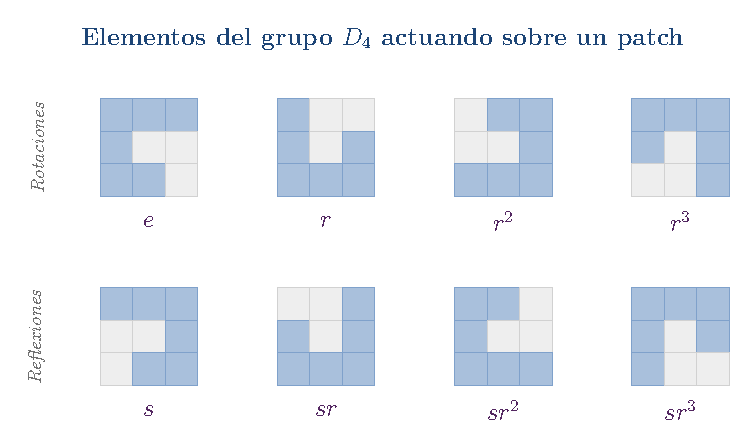
\includegraphics[width=0.85\textwidth]{images/d4_group_actions}
	\caption[Elements of the group $D_4$ acting on a patch]{The 8 elements of the dihedral group $D_4$ acting on an asymmetric patch. Top row: the 4 rotations ($e$, $r$, $r^2$, $r^3$). Bottom row: the 4 reflections ($s$, $sr$, $sr^2$, $sr^3$). The $D_4$-equivariant network produces the same output regardless of the applied transformation.}
	\label{fig:d4_group_actions}
\end{figure}

\subsubsection{Mathematical Verification of Equivariance}\label{subsubsec:verificacion_matematica_equivarianza}

The theoretical correctness of equivariant architectures must be complemented with rigorous methods of mathematical verification that validate the fundamental property of equivariance.

\begin{definition}[Equivariance Error Measure]\label{def:error_equivarianza}
For a function $\Phi$ and a group $G$, we define the \textit{equivariance error measure} as:
\begin{equation}
\mathcal{E}_G(\Phi, x) = \frac{1}{|G|} \sum_{g \in G} \|\Phi(g \cdot x) - g \cdot \Phi(x)\|^2
\end{equation}
where $\|\cdot\|$ is an appropriate norm in the output space.
\end{definition}

\begin{theorem}[Equivariance Criterion]\label{thm:criterio_equivarianza}
A function $\Phi$ is $G$-equivariant if and only if $\mathcal{E}_G(\Phi, x) = 0$ for every input $x$ in the domain.
\end{theorem}

\begin{proof}
$(\Rightarrow)$ If $\Phi$ is $G$-equivariant, then $\Phi(g \cdot x) = g \cdot \Phi(x)$ for all $g \in G$, which implies $\|\Phi(g \cdot x) - g \cdot \Phi(x)\|^2 = 0$ for all $g$. Therefore, $\mathcal{E}_G(\Phi, x) = \frac{1}{|G|} \sum_{g \in G} 0 = 0$.

$(\Leftarrow)$ If $\mathcal{E}_G(\Phi, x) = 0$, then $\sum_{g \in G} \|\Phi(g \cdot x) - g \cdot \Phi(x)\|^2 = 0$. Since each summand is non-negative (squared norm), they must all be zero: $\|\Phi(g \cdot x) - g \cdot \Phi(x)\|^2 = 0$ for all $g \in G$. By the positive definiteness of the norm, $\Phi(g \cdot x) = g \cdot \Phi(x)$ for all $g \in G$, that is, $\Phi$ is $G$-equivariant.
\end{proof}

\begin{proposition}[Error Propagation]\label{prop:propagacion_error}
For the composition of functions $\Phi = \Phi_n \circ \cdots \circ \Phi_1$, where each $\Phi_i$ has Lipschitz constant $L_i$ and $x_i = (\Phi_{i-1} \circ \cdots \circ \Phi_1)(x)$ are the intermediate activations (with $x_0 = x$), the maximum equivariance deviation at each layer propagates as:
\begin{equation}
\sup_{g \in G}\|\Phi(g \cdot x) - g \cdot \Phi(x)\| \leq \sum_{i=1}^{n} \left(\prod_{j=i+1}^{n} L_j\right) \sup_{g \in G}\|\Phi_i(g \cdot x_i) - g \cdot \Phi_i(x_i)\|
\end{equation}
where the empty product (when $i = n$) equals $1$.
\end{proposition}

\begin{proof}
For $n = 1$ the inequality is trivial. For the inductive step, let $\Psi = \Phi_{n-1} \circ \cdots \circ \Phi_1$. Fixing $g \in G$, we write:
\begin{align}
\|\Phi(g \cdot x) - g \cdot \Phi(x)\| &= \|\Phi_n(\Psi(g \cdot x)) - g \cdot \Phi_n(\Psi(x))\| \\
&\leq \|\Phi_n(\Psi(g \cdot x)) - \Phi_n(g \cdot \Psi(x))\| + \|\Phi_n(g \cdot \Psi(x)) - g \cdot \Phi_n(\Psi(x))\|
\end{align}
The first term is bounded by the Lipschitz property: $L_n \|\Psi(g \cdot x) - g \cdot \Psi(x)\|$. The second is the equivariance deviation of $\Phi_n$ evaluated at $x_n = \Psi(x)$. Taking the supremum over $g$ and applying the inductive hypothesis to $\Psi$ yields the desired bound.
\end{proof}

\begin{definition}[Practical Equivariance]\label{cor:tolerancia_error}
In numerical implementations with finite precision, a function is considered \textit{practically equivariant} if:
\begin{equation}
\mathcal{E}_G(\Phi, x) < \epsilon
\end{equation}
where $\epsilon$ is an appropriate tolerance (typically $\epsilon \sim 10^{-6}$ for floating-point precision).
\end{definition}

\paragraph{Analysis of Mathematical Precision}

The theoretical analysis of equivariance precision reveals that architectures based on group theory maintain exact equivariance properties, subject only to numerical precision limitations.

\begin{remark}[Numerical Stability of Equivariance]\label{rem:estabilidad_numerica}
For a $D_4$-equivariant architecture implemented with finite-precision arithmetic, the equivariance error is of the order:
\begin{equation}
\sup_{g \in G}\|\Phi(g \cdot x) - g \cdot \Phi(x)\| = O\!\left(\epsilon_{\text{mach}} \cdot \text{depth}(\Phi) \cdot \|x\|\right)
\end{equation}
where $\epsilon_{\text{mach}}$ is the machine precision and $\text{depth}(\Phi)$ is the depth of the network. This heuristic estimate reflects that each layer introduces a rounding error proportional to $\epsilon_{\text{mach}}$, and these errors accumulate linearly across the layers of the network, analogously to the standard analysis of error propagation in floating-point arithmetic.
\end{remark}

\textbf{Mathematical Meaning of the Errors.} The observed errors of the order of $10^{-6}$ in numerical implementations are consistent with the expected precision of 32-bit floating-point arithmetic, confirming that the theoretical equivariance is preserved up to the limiting precision of the hardware.

In particular, when the numerical precision tends to zero ($\epsilon_{\text{mach}} \to 0$), the implementations converge toward exact equivariance, since the equivariance error tends to zero with $\epsilon_{\text{mach}}$.

This theoretical grounding demonstrates how the abstract concepts of group theory materialize in mathematically rigorous architectures, providing the conceptual basis for addressing more complex groups in the following subsections.

\subsection[GCNNs for Finite Groups]{\glspl{GCNN} for Finite Groups}\label{subsec:gcnns_grupos_finitos}

The application of the theory of group convolutions to finite groups represents one of the most direct and computationally tractable extensions of classical \glspl{CNN}. Finite groups appear naturally in many computer vision domains, where discrete symmetries such as rotations by multiples of 90 degrees or reflections are relevant to the interpretation of the data.

\subsubsection{Finite Groups in Computer Vision}

In the context of image processing, the most relevant finite groups are those that preserve the discrete grid structure while incorporating significant geometric symmetries.

\begin{definition}[Cyclic Group of Rotations]
The cyclic group $C_4 = \{e, r, r^2, r^3\}$ represents the rotations by multiples of $90^\circ$ in the plane, where $r$ denotes a $90^\circ$ counterclockwise rotation and $e$ is the identity.
\end{definition}

\begin{definition}[Dihedral Group of the Square]
The dihedral group $D_4 = \{e, r, r^2, r^3, s, sr, sr^2, sr^3\}$ includes the four rotations of $C_4$ plus four reflections $s, sr, sr^2, sr^3$, where $s$ represents a reflection about an axis.
\end{definition}

These groups are particularly important because:
\begin{itemize}
    \item \textbf{Grid preservation}: The transformations maintain the discrete pixel structure
    \item \textbf{Practical relevance}: Many textures and patterns exhibit these symmetries
    \item \textbf{Computational efficiency}: The finite number of elements allows exact implementations
\end{itemize}

The most common symmetry groups in practical applications are:

\begin{table}[h]
\centering
\begin{tabular}{|l|c|l|l|}
\hline
\textbf{Group} & \textbf{Order} & \textbf{Elements} & \textbf{Applications} \\
\hline
$C_4$ (p4) & 4 & Rotations $0^\circ, 90^\circ, 180^\circ, 270^\circ$ & Textures, regular patterns \\
$D_4$ (p4m) & 8 & Rotations + reflections & Symmetric objects, crystals \\
$C_2$ & 2 & Identity, $180^\circ$ rotation & Bilateral symmetry \\
$D_2$ & 4 & Identity + 3 reflections & Shape analysis \\
\hline
\end{tabular}
\caption{Common finite groups in computer vision}
\label{tab:grupos_finitos}
\end{table}

\subsubsection[Construction of GCNNs for Discrete Groups]{Construction of \glspl{GCNN} for Discrete Groups}

The construction of a \gls{GCNN} for a finite group $G$ follows the theoretical framework established in \autoref{subsec:fundamentos_teoricos}, but exploits the discrete structure for significant computational simplifications.

\paragraph{Lifting from the Input Space}

The first layer of a \gls{GCNN} must transform functions defined on the Euclidean space $\mathbb{R}^2$ (or its discretization) into functions defined over the group $G$. This operation is called \textbf{lifting}.

\begin{definition}[Lifting Convolution]
For an input image $f: \mathbb{Z}^2 \to \mathbb{R}$ and a filter $\psi: \mathbb{Z}^2 \to \mathbb{R}$, the lifting convolution produces a function on $G$ defined by:
\begin{equation}
(f \star \psi)(g) = \sum_{x \in \mathbb{Z}^2} f(x) \psi(g^{-1} \cdot x)
\label{eq:lifting_convolution}
\end{equation}
where $g \in G$ and the sum is over a local window.
\end{definition}

For the group $C_4$, this means that for each spatial position and each rotation $g \in \{e, r, r^2, r^3\}$, we compute the response of the filter rotated by $g^{-1}$.

\paragraph{Group Convolutions in Intermediate Layers}

The subsequent layers operate on functions $f: G \to \mathbb{R}^C$ (where $C$ is the number of channels) using full group convolutions:

\begin{equation}
(f \star_G \psi)(u) = \sum_{g \in G} f(g) \psi(u^{-1}g)
\label{eq:group_conv_discrete}
\end{equation}

\begin{algorithm}[h]
\caption{G-CNN Convolution for a Finite Group}
\label{alg:gcnn_finite}
\begin{algorithmic}[1]
\Require Input function $f$, filters $\{\psi_i\}$, group $G = \{g_1, \ldots, g_n\}$
\Ensure Feature map $\text{output}$
\State Initialize $\text{output}$ with dimensions $(|G|, H, W, C_{\text{out}})$
\For{each filter $i$ in $\{1, \ldots, C_{\text{out}}\}$}
    \For{each group element $u \in G$}
        \For{each position $(h, w)$}
            \State $\text{sum} \leftarrow 0$
            \For{each group element $g \in G$}
                \For{each channel $c$ in input}
                    \State $\text{sum} \leftarrow \text{sum} + f[g][h][w][c] \cdot \psi_i[u^{-1}g][c]$
                \EndFor
            \EndFor
            \State $\text{output}[u][h][w][i] \leftarrow \text{sum}$
        \EndFor
    \EndFor
\EndFor
\Return $\text{output}$
\end{algorithmic}
\end{algorithm}

\subsubsection{Mathematical Theory for the Rotation Group $C_4$}

The cyclic group $C_4 = \{e, r, r^2, r^3\}$ provides a fundamental case for understanding the mathematical structure of group convolutions.

\paragraph{Structure of the Feature Space}

The feature maps in a $C_4$-CNN form a vector space $\mathcal{V} = \mathbb{R}^{C_4 \times \Omega \times \mathbb{R}^C}$, where:
\begin{itemize}
    \item $C_4$: Group space with 4 elements
    \item $\Omega \subset \mathbb{Z}^2$: Discrete spatial domain
    \item $\mathbb{R}^C$: Feature channel space
\end{itemize}

\begin{definition}[Action of $C_4$ on Filters]
The action of the group $C_4$ on filters $\psi: \mathbb{Z}^2 \to \mathbb{R}$ is defined via the matrix representation of rotations:
\begin{equation}
(r^k \cdot \psi)(i,j) = \psi(R_k^{-1} \cdot (i,j))
\end{equation}
where $R_k$ is the rotation matrix by $k \cdot 90^\circ$:
\begin{equation}
R_k = \begin{pmatrix}
\cos(k\pi/2) & -\sin(k\pi/2) \\
\sin(k\pi/2) & \cos(k\pi/2)
\end{pmatrix}
\end{equation}
\end{definition}

\begin{theorem}[Parametric Efficiency of $C_4$-CNNs]
A $C_4$-CNN requires exactly $1/4$ of the parameters that a standard CNN requires to represent the same space of $C_4$-equivariant functions, due to the parameter sharing induced by the group structure.
\end{theorem}

\begin{proof}
In a standard CNN, each filter $\psi: \mathbb{Z}^2 \to \mathbb{R}$ has independent parameters for each kernel position. In a $C_4$-CNN, equivariance requires that the 4 rotated versions of the filter $\{\psi, r \cdot \psi, r^2 \cdot \psi, r^3 \cdot \psi\}$ be generated from the same set of base parameters $\psi$. To represent a $C_4$-equivariant function, a standard CNN would need 4 independent filters (one for each orientation), with a total of $4P$ parameters (where $P$ is the kernel size). The $C_4$-CNN uses a single base filter with $P$ parameters and generates the other 3 via the group action, reaching the same function space with $P = (4P)/4$ parameters.
\end{proof}

\subsubsection{Theory of the Dihedral Group $D_4$}

The extension to the dihedral group $D_4$ incorporates reflections in addition to rotations, significantly enriching the algebraic structure.

\paragraph{Mathematical Structure of Reflections}

The reflections in $D_4$ are characterized by orthogonal linear transformations with determinant $-1$:

\begin{definition}[Matrix Representation of Reflections in $D_4$]
The fundamental reflections are expressed as:
\begin{align}
s_h: \begin{pmatrix} x \\ y \end{pmatrix} &\mapsto \begin{pmatrix} 1 & 0 \\ 0 & -1 \end{pmatrix} \begin{pmatrix} x \\ y \end{pmatrix} = \begin{pmatrix} x \\ -y \end{pmatrix} \\
s_v: \begin{pmatrix} x \\ y \end{pmatrix} &\mapsto \begin{pmatrix} -1 & 0 \\ 0 & 1 \end{pmatrix} \begin{pmatrix} x \\ y \end{pmatrix} = \begin{pmatrix} -x \\ y \end{pmatrix} \\
s_d: \begin{pmatrix} x \\ y \end{pmatrix} &\mapsto \begin{pmatrix} 0 & 1 \\ 1 & 0 \end{pmatrix} \begin{pmatrix} x \\ y \end{pmatrix} = \begin{pmatrix} y \\ x \end{pmatrix}
\end{align}
\end{definition}

\paragraph{Complete Algebraic Structure}

The multiplication table of $D_4$ encodes the complete algebraic structure of the group:

\begin{table}[h]
\centering
\small
\begin{tabular}{|c|c|c|c|c|c|c|c|c|}
\hline
$\cdot$ & $e$ & $r$ & $r^2$ & $r^3$ & $s$ & $sr$ & $sr^2$ & $sr^3$ \\
\hline
$e$ & $e$ & $r$ & $r^2$ & $r^3$ & $s$ & $sr$ & $sr^2$ & $sr^3$ \\
$r$ & $r$ & $r^2$ & $r^3$ & $e$ & $sr$ & $sr^2$ & $sr^3$ & $s$ \\
$r^2$ & $r^2$ & $r^3$ & $e$ & $r$ & $sr^2$ & $sr^3$ & $s$ & $sr$ \\
$r^3$ & $r^3$ & $e$ & $r$ & $r^2$ & $sr^3$ & $s$ & $sr$ & $sr^2$ \\
$s$ & $s$ & $sr^3$ & $sr^2$ & $sr$ & $e$ & $r^3$ & $r^2$ & $r$ \\
$sr$ & $sr$ & $s$ & $sr^3$ & $sr^2$ & $r$ & $e$ & $r^3$ & $r^2$ \\
$sr^2$ & $sr^2$ & $sr$ & $s$ & $sr^3$ & $r^2$ & $r$ & $e$ & $r^3$ \\
$sr^3$ & $sr^3$ & $sr^2$ & $sr$ & $s$ & $r^3$ & $r^2$ & $r$ & $e$ \\
\hline
\end{tabular}
\caption{Multiplication table of the dihedral group $D_4$}
\label{tab:d4_multiplication}
\end{table}

\subsubsection{Fundamental Theoretical Considerations}

\paragraph{Dimensionality Analysis}

The dimensional scaling by the factor $|G|$ has profound theoretical implications for expressive capacity:

\begin{remark}[Dimensionality-Expressivity Trade-off]\label{thm:tradeoff_dimensional}
For a G-CNN that processes functions over $G \times \Omega$, the dimension of the feature space scales as $|G| \cdot \text{dim}(\Omega) \cdot C$. However, the weight sharing induced by equivariance reduces the number of free parameters. Intuitively, if the data possess additional symmetries (that is, the stabilizer $\text{Stab}(x) = \{g \in G : g \cdot x = x\}$ is non-trivial for typical inputs), the effective dimension of the parameter space is further reduced. By the orbit-stabilizer theorem, $|G| = |\text{Orb}(x)| \cdot |\text{Stab}(x)|$, which heuristically suggests that the effective dimension is of the order of $|\text{Orb}(x)| \cdot \text{dim}(\Omega) \cdot C$ rather than $|G| \cdot \text{dim}(\Omega) \cdot C$.
\end{remark}

\paragraph{Implicit Geometric Regularization}

Equivariance induces a natural form of regularization:

\begin{remark}[Regularization by Equivariance]\label{prop:regularizacion_equivarianza}
In architectures where equivariance is not built in by construction, it can be imposed as a soft constraint via the penalty:
\begin{equation}
\mathcal{R}_{\text{equiv}} = \frac{1}{|G|} \sum_{g \in G} \|\theta - g \cdot \theta\|^2
\end{equation}
where $g \cdot \theta$ denotes the transformation of parameters under the action of $g$. Note that $\mathcal{R}_{\text{equiv}} = 0$ if and only if $\theta = g \cdot \theta$ for all $g \in G$, which corresponds exactly to the weight sharing that defines an equivariant layer. The penalty $\mathcal{R}_{\text{equiv}}$ acts as a continuous relaxation of this constraint: minimizing it encourages the parameters to approach the subspace of shared weights, thereby reducing the effective capacity of the model analogously to an $L_2$ regularization.
\end{remark}

\subsubsection{Theoretical Foundations of the Empirical Advantages}

\paragraph{Experiments in Texture Recognition}

The experiments of Cohen and Welling~\citep{cohen2016groupequivariantconvolutional} on the \textit{rotated CIFAR-10} dataset demonstrate significant improvements:

\begin{table}[h]
\centering
\begin{tabular}{|l|c|c|}
\hline
\textbf{Model} & \textbf{CIFAR-10} & \textbf{Rotated CIFAR-10} \\
\hline
Standard CNN & 92.3\% & 47.2\% \\
\gls{GCNN} ($C_4$) & 92.8\% & 71.8\% \\
\gls{GCNN} ($D_4$) & 93.1\% & 73.4\% \\
\hline
\end{tabular}
\caption{Recognition accuracy with arbitrary rotations}
\label{tab:resultados_rotaciones}
\end{table}

\paragraph{Analysis of Crystallographic Patterns}

In materials science applications, \glspl{GCNN} have shown advantages in the analysis of crystal structures that exhibit symmetries specific to the corresponding space group~\citep{weiler2018learningsteerable}.

\paragraph{Medical Segmentation}

In medical imaging, where the orientation of the patient can vary, \glspl{GCNN} provide automatic robustness without the need for extensive data augmentation.

\subsubsection{Limitations and Considerations}

\paragraph{Computational Scalability}

The computational cost scales linearly with $|G|$:
\begin{equation}
\text{FLOPs}_{\text{G-CNN}} = |G| \times \text{FLOPs}_{\text{CNN}}
\end{equation}

For large groups, this can be prohibitive in applications with real-time constraints.

\paragraph{Approximate Symmetries}

In real data, symmetries are often approximate. \glspl{GCNN} can be sensitive to deviations from exact symmetry, requiring care in the selection of the appropriate group.

\paragraph{Compatibility with Existing Architectures}

Integration with techniques such as attention, skip connections, or batch normalization requires careful adaptations to preserve equivariance.

\subsubsection{Extensions and Future Directions}

\paragraph{More General Finite Groups}

The extension to symmetry groups of regular polyhedra (tetrahedral, octahedral, icosahedral) opens up applications in 3D data analysis and computational chemistry.

\paragraph{Combination with Other Symmetries}

The composition of discrete symmetries with continuous symmetries (such as scaling) represents an active area of research.

\paragraph{Symmetry Learning}

Emerging methods seek to automatically discover the relevant symmetries instead of specifying them a priori, combining \glspl{GCNN} with representation learning techniques.

\glspl{GCNN} for finite groups represent a mature and practical extension of classical convolutions, providing theoretically guaranteed robustness to discrete symmetries common in computer vision applications. Their relatively straightforward implementation and their demonstrated benefits make them a valuable tool for domains where discrete symmetries are relevant. Understanding these principles establishes the basis for extensions to more complex groups, as we will see in the following subsections on spherical convolutions and convolutions on manifolds.


Steerable \glspl{CNN} represent a natural extension of discrete \glspl{GCNN} toward the continuous regime, preserving the theoretical guarantees of equivariance while providing greater representational flexibility. Their formulation based on representation theory provides an elegant mathematical framework that connects classical harmonic analysis with modern deep learning architectures.

\subsection{Compact Continuous Groups (SO(2), SO(3))}\label{subsec:grupos_continuos_compactos}

The compact continuous groups $SO(2)$ and $SO(3)$ represent fundamental extensions that allow exact equivariance to continuous rotations in 2D and 3D respectively. This subsection examines the specialized architectures that exploit these rotational symmetries, from Steerable CNNs for SO(2) to spherical CNNs and sophisticated extensions that incorporate scales and irregular structures.

\subsubsection{The Group SO(2): Continuous 2D Rotations and Steerable CNNs}\label{subsubsec:steerable_cnns_so2}

The transition from finite groups of discrete rotations (such as $C_4$ or $D_4$ studied in \autoref{subsec:gcnns_grupos_finitos}) to the continuous rotation group $SO(2)$ represents one of the most significant advances in the development of geometrically aware architectures. While \glspl{GCNN} for finite groups provide equivariance to a discrete set of transformations, Steerable CNNs allow equivariance to continuous rotations, offering a richer and more flexible representation of rotational symmetries.

\paragraph{Motivation: Limitations of Discretizations}

\glspl{GCNN} for finite groups, although powerful, present inherent limitations when the natural symmetries of the data do not align perfectly with the discrete transformations of the group.

\begin{example}[Limitation of $C_4$ on Natural Data]
Consider an image that contains an object rotated by $45^{\circ}$. A \gls{GCNN} based on $C_4$ ($90^{\circ}$ rotations) cannot capture this exact orientation, producing suboptimal responses that are interpolations between the available discrete orientations.
\end{example}

Discretization introduces rotational \textit{aliasing} effects, where intermediate rotations are poorly approximated by the nearest discrete orientations:

\begin{equation}
\text{Error}(\theta) = \min_{k} |\theta - k \cdot \frac{2\pi}{|G|}|
\end{equation}

For $C_4$, this error can reach up to $45^{\circ}$, which represents a significant approximation for many practical applications.

\paragraph{The Continuous Rotation Group SO(2)}

The special orthogonal group $SO(2)$ consists of all rotations in the plane about the origin:

\begin{definition}[Group SO(2)]
$SO(2) = \{R_\theta : \theta \in [0, 2\pi)\}$ where each element $R_\theta$ is the rotation matrix:
\begin{equation}
R_\theta = \begin{pmatrix}
\cos \theta & -\sin \theta \\
\sin \theta & \cos \theta
\end{pmatrix}
\end{equation}
\end{definition}

\begin{proposition}[Properties of SO(2)]
The group $SO(2)$ is:
\begin{enumerate}
    \item \textbf{Compact}: Topologically equivalent to $S^1$
    \item \textbf{Abelian}: $R_\alpha R_\beta = R_{\alpha + \beta} = R_\beta R_\alpha$
    \item \textbf{One-parameter}: Parametrized by a single angle $\theta$
\end{enumerate}
\end{proposition}

\begin{proof}
(1) \textit{Compact}: $SO(2) = \{R_\theta : \theta \in [0, 2\pi)\}$ with $R_\theta = \begin{psmallmatrix} \cos\theta & -\sin\theta \\ \sin\theta & \cos\theta \end{psmallmatrix}$. The map $\theta \mapsto R_\theta$ is a homeomorphism between $[0, 2\pi) / (0 \sim 2\pi)$ and $SO(2)$, identifying it with $S^1$. Since $S^1$ is closed and bounded in $\mathbb{R}^2$, it is compact by Heine-Borel.

(2) \textit{Abelian}: $R_\alpha R_\beta$ corresponds to the rotation by angle $\alpha + \beta$ (composition of rotations in the plane). Since addition in $\mathbb{R}/2\pi\mathbb{Z}$ is commutative, $R_\alpha R_\beta = R_{\alpha+\beta} = R_{\beta+\alpha} = R_\beta R_\alpha$.

(3) \textit{One-parameter}: $\dim(SO(2)) = 1$, since the condition $R^TR = I$ with $\det R = 1$ imposes 3 independent constraints on the 4 parameters of a $2 \times 2$ matrix, leaving $4 - 3 = 1$ degree of freedom.
\end{proof}

This structure allows the use of \textbf{circular harmonic analysis} to construct efficient representations of equivariant functions.

\paragraph{Theory of Steerable Filters}

Steerable filters constitute the theoretical foundation of Steerable CNNs, allowing responses to arbitrary rotations to be generated from a base set of filters.

\begin{figure}[htbp]
	\centering
	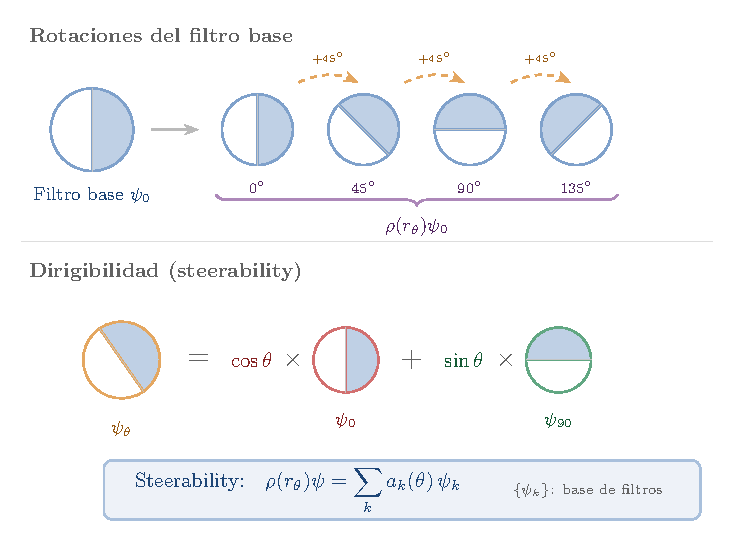
\includegraphics[width=0.85\textwidth]{images/steerable_filters}
	\caption[Steerable filters and steerability]{Steerable filters: any rotation of the base filter $\psi_0$ can be expressed as a linear combination of filters from a finite basis. This property allows equivariance to continuous rotations with a finite number of parameters.}
	\label{fig:steerable_filters}
\end{figure}

\begin{definition}[Steerable Filter]
A filter $h: \mathbb{R}^2 \to \mathbb{R}$ is \textbf{steerable} of order $N$ if there exist base filters $\{h_0, h_1, \ldots, h_{N-1}\}$ and interpolation functions $\{k_n(\theta)\}_{n=0}^{N-1}$ such that:
\begin{equation}
h_\theta(x, y) = \sum_{n=0}^{N-1} k_n(\theta) h_n(x, y)
\end{equation}
where $h_\theta$ is the version of the base filter rotated by angle $\theta$.
\end{definition}

The theory of circular harmonics provides a natural basis for constructing steerable filters:

\begin{theorem}[Representation by Circular Harmonics]
Every function $f: S^1 \to \mathbb{C}$ (where $S^1$ represents orientations) admits a Fourier series expansion:
\begin{equation}
f(\theta) = \sum_{k=-\infty}^{\infty} c_k e^{ik\theta}
\end{equation}
The coefficients $c_k$ transform simply under rotations: if $g_\phi(\theta) = f(\theta + \phi)$, then the coefficients of $g_\phi$ are $c_k e^{ik\phi}$.
\end{theorem}

\begin{proof}
The Fourier series expansion of $f$ is a consequence of the completeness of the orthonormal system $\{e^{ik\theta}\}_{k \in \mathbb{Z}}$ in $L^2(S^1)$, with $\langle e^{ik\theta}, e^{il\theta} \rangle = \frac{1}{2\pi}\int_0^{2\pi} e^{i(k-l)\theta} d\theta = \delta_{kl}$. The coefficients are computed as $c_k = \frac{1}{2\pi}\int_0^{2\pi} f(\theta) e^{-ik\theta} d\theta$. For the transformation under rotations, if $g_\phi(\theta) = f(\theta + \phi)$, its coefficients are:
\[
\hat{g}_k = \frac{1}{2\pi}\int_0^{2\pi} f(\theta + \phi) e^{-ik\theta} d\theta = \frac{1}{2\pi}\int_0^{2\pi} f(\alpha) e^{-ik(\alpha - \phi)} d\alpha = e^{ik\phi} c_k
\]
where the substitution $\alpha = \theta + \phi$ and the periodicity of the integral were used.
\end{proof}

\begin{definition}[Circular Harmonic Filter]
A circular harmonic filter of frequency $k$ in polar coordinates $(r, \theta)$ is defined as:
\begin{equation}
\psi_k(r, \theta) = R_k(r) e^{ik\theta}
\end{equation}
where $R_k(r)$ is the radial part and $e^{ik\theta}$ is the angular part.
\end{definition}

\paragraph{Architecture of Steerable CNNs}

The construction of Steerable CNNs follows the framework developed by Weiler and Welling~\citep{weiler2019general}, generalizing the principles of group equivariance to continuous representations.

Instead of discretizing orientations, Steerable CNNs operate on \textbf{geometric fields} that transform according to irreducible representations of $SO(2)$.

\begin{definition}[Geometric Field]
A geometric field of type $\rho$ is a function $f: \mathbb{R}^2 \to V$ where $V$ is a vector space equipped with a representation $\rho: SO(2) \to GL(V)$ such that:
\begin{equation}
(g \cdot f)(x) = \rho(g) f(g^{-1} x)
\end{equation}
for all $g \in SO(2)$.
\end{definition}

\begin{definition}[Irreducible Representations of SO(2)]\label{def:irreps_so2}
The \textit{irreducible representations} of $SO(2)$ are classified by integers $k \in \mathbb{Z}$:

\begin{equation}
\rho_k(R_\theta) = e^{ik\theta} \quad \text{for } k \neq 0
\end{equation}

and the trivial representation for $k = 0$: $\rho_0(R_\theta) = 1$.

For real representations, frequencies $\pm k$ are combined:
\begin{equation}
\rho_k^{\text{real}}(R_\theta) = \begin{pmatrix}
\cos(k\theta) & -\sin(k\theta) \\
\sin(k\theta) & \cos(k\theta)
\end{pmatrix}
\end{equation}
\end{definition}

\paragraph{Applications in Natural Image Analysis}

Steerable CNNs have demonstrated superiority in tasks where exact orientation is critical:

\begin{itemize}
    \item \textbf{Fiber analysis}: In medical images of connective tissue
    \item \textbf{Fingerprint recognition}: Where ridges have precise orientations
    \item \textbf{Materials analysis}: Detection of cracks and structural defects
\end{itemize}

Experiments on datasets augmented with continuous rotations show consistent advantages over discrete approaches, providing a natural transition toward more complex groups such as $SO(3)$ for three-dimensional data.

\subsubsection{Practical Implementation of Steerable CNNs for SO(2)}\label{subsubsec:implementacion_steerable_cnns}

The transition from the theory of steerable filters to efficient computational implementations requires addressing several technical challenges specific to the continuous group $SO(2)$. Unlike finite groups, where transformations are discrete and exact, Steerable CNNs must handle continuous rotations using finite-dimensional representations.

\paragraph{Irreducible Representations of SO(2)}

The practical implementation begins with the explicit construction of the irreducible representations:

The irreducible representations of $SO(2)$ are implemented mathematically as already defined in \autoref{def:irreps_so2}.

\paragraph{Generation of Circular Harmonic Filters}

The core of Steerable CNNs lies in the generation of base filters using circular harmonics:

\begin{listing}[h]
\begin{lstlisting}[language=Python]
class CircularHarmonics:
    """Circular harmonics for SO(2) steerable filters."""

    @staticmethod
    def generate_filter_basis(size: int, max_frequency: int,
                             sigma: float = 0.5) -> torch.Tensor:
        """Generate basis of circular harmonic filters."""
        # Create coordinate grid
        coords = torch.linspace(-1, 1, size)
        y, x = torch.meshgrid(coords, coords, indexing='ij')

        # Convert to polar coordinates
        r = torch.sqrt(x**2 + y**2)
        theta = torch.atan2(y, x)

        # Gaussian radial envelope
        radial_envelope = torch.exp(-0.5 * (r / sigma) ** 2)

        # Generate basis functions
        basis_filters = []

        # k=0 (trivial representation)
        basis_0 = radial_envelope
        basis_filters.append(basis_0)

        # k>0 (non-trivial representations)
        for k in range(1, max_frequency + 1):
            # Cosine component
            cos_k = radial_envelope * torch.cos(k * theta)
            basis_filters.append(cos_k)

            # Sine component
            sin_k = radial_envelope * torch.sin(k * theta)
            basis_filters.append(sin_k)

        return torch.stack(basis_filters)

    @staticmethod
    def rotate_harmonics(harmonics: torch.Tensor, angle: float,
                        max_frequency: int) -> torch.Tensor:
        """Rotate circular harmonics by a given angle."""
        result = harmonics.clone()

        # k=0 unchanged
        # k>0 components
        idx = 1
        for k in range(1, max_frequency + 1):
            # Extract cosine and sine components
            cos_comp = harmonics[idx]
            sin_comp = harmonics[idx + 1]

            # Apply rotation matrix
            c = math.cos(k * angle)
            s = math.sin(k * angle)

            result[idx] = c * cos_comp - s * sin_comp
            result[idx + 1] = s * cos_comp + c * sin_comp

            idx += 2

        return result
\end{lstlisting}
\caption{Generation and rotation of circular harmonics}
\label{code:circular_harmonics}
\end{listing}

\paragraph{Steerable Convolutional Layer}

The implementation of the steerable convolution combines the base filters with learnable coefficients:

\begin{listing}[h]
\begin{lstlisting}[language=Python]
class SteerableConv2d(nn.Module):
    """2D steerable convolution layer for SO(2) equivariance."""

    def __init__(self, in_irreps: SO2_Irreps, out_irreps: SO2_Irreps,
                 kernel_size: int, max_frequency: int = 4):
        super().__init__()

        self.in_irreps = in_irreps
        self.out_irreps = out_irreps
        self.kernel_size = kernel_size
        self.max_frequency = max_frequency

        # Generate harmonic basis
        self.register_buffer(
            'basis_filters',
            CircularHarmonics.generate_filter_basis(
                kernel_size, max_frequency
            )
        )

        num_basis = self.basis_filters.shape[0]

        # Learnable coefficients to combine basis functions
        self.coefficients = nn.Parameter(
            torch.randn(out_irreps.dim(), in_irreps.dim(), num_basis)
        )

        self.reset_parameters()

    def reset_parameters(self):
        """Initialize parameters."""
        std = math.sqrt(2.0 / (self.in_irreps.dim() + self.out_irreps.dim()))
        nn.init.normal_(self.coefficients, 0, std)

    def forward(self, x: torch.Tensor) -> torch.Tensor:
        """Forward pass of steerable convolution."""
        # Generate steerable kernels
        kernels = self._generate_kernels()  # (out_dim, in_dim, K, K)

        # Apply convolution
        output = F.conv2d(x, kernels, padding=self.kernel_size//2)

        return output

    def _generate_kernels(self) -> torch.Tensor:
        """Generate steerable kernels from basis functions."""
        # Combine basis functions with learned coefficients
        kernels = torch.einsum(
            'oib,bkl->oikl',
            self.coefficients,
            self.basis_filters
        )

        return kernels
\end{lstlisting}
\caption{Implementation of steerable convolution}
\label{code:steerable_conv}
\end{listing}

\paragraph{Equivariant Activation Functions}

A critical aspect of Steerable CNNs is the design of activation functions that preserve the structure of irreducible representations:

\begin{listing}[h]
\begin{lstlisting}[language=Python]
def steerable_relu(x: torch.Tensor, irreps: SO2_Irreps) -> torch.Tensor:
    """ReLU that preserves irrep structure."""
    result = []
    channel_idx = 0

    for freq, mult in irreps.irreps:
        if freq == 0:
            # Trivial representation - standard ReLU
            channels = x[:, channel_idx:channel_idx+mult]
            result.append(F.relu(channels))
        else:
            # Non-trivial representation - norm-ReLU
            channels = x[:, channel_idx:channel_idx+mult]  # (N, 2, H, W)

            # Compute norm
            norm = torch.norm(channels, dim=1, keepdim=True)  # (N, 1, H, W)

            # Apply gating
            gated_norm = F.relu(norm)

            # Normalize and scale
            eps = 1e-8
            unit_channels = channels / (norm + eps)
            result.append(unit_channels * gated_norm)

        channel_idx += mult

    return torch.cat(result, dim=1)
\end{lstlisting}
\caption{Activation function that preserves equivariance}
\label{code:steerable_relu}
\end{listing}

\paragraph{Complete SO(2)-CNN Architecture}

The combination of all the components makes it possible to construct a CNN that is fully equivariant to continuous rotations:

\begin{listing}[h]
\begin{lstlisting}[language=Python]
class SO2SteerableCNN(nn.Module):
    """Fully steerable CNN for SO(2)."""

    def __init__(self, num_classes: int = 10, max_frequency: int = 3):
        super().__init__()

        self.max_frequency = max_frequency

        # Define irreps progression
        self.irreps_hidden = SO2_Irreps(max_frequency)

        # Lifting layer: R^2 -> SO(2)
        self.lift = nn.Conv2d(3, self.irreps_hidden.dim() * 16,
                              kernel_size=3, padding=1)

        # Steerable layers
        self.steerable1 = SteerableLayer(
            self.irreps_hidden, self.irreps_hidden,
            kernel_size=3, padding=1
        )

        self.steerable2 = SteerableLayer(
            self.irreps_hidden, self.irreps_hidden,
            kernel_size=3, padding=1
        )

        # Pooling and classification
        self.pool = nn.MaxPool2d(2, 2)
        self.adaptive_pool = nn.AdaptiveAvgPool2d(1)

        hidden_dim = self.irreps_hidden.dim() * 16
        self.classifier = nn.Sequential(
            nn.Linear(hidden_dim, 128),
            nn.ReLU(),
            nn.Dropout(0.5),
            nn.Linear(128, num_classes)
        )

    def forward(self, x: torch.Tensor) -> torch.Tensor:
        # Lifting
        x = F.relu(self.lift(x))
        x = self.pool(x)

        # Steerable convolutions
        x = self.steerable1(x)
        x = self.pool(x)

        x = self.steerable2(x)

        # Global pooling
        x = self.adaptive_pool(x)
        x = x.view(x.size(0), -1)

        # Classification
        x = self.classifier(x)

        return x
\end{lstlisting}
\caption{Complete SO(2) Steerable CNN architecture}
\label{code:so2_steerable_cnn}
\end{listing}

\paragraph{Equivariance Verification for Continuous Rotations}

Empirical verification for continuous groups requires sampling rotations from the continuum:

\begin{listing}[h]
\begin{lstlisting}[language=Python]
def test_continuous_equivariance(model: nn.Module, x: torch.Tensor,
                               angles: List[float] = None) -> Dict[str, float]:
    """Test equivariance for continuous rotations."""
    if angles is None:
        angles = [0, np.pi/4, np.pi/2, np.pi, 3*np.pi/2]

    model.eval()
    results = {}

    with torch.no_grad():
        # Original output
        original_output = model(x)

        for angle in angles:
            # Rotate input using bilinear interpolation
            rotated_x = rotate_tensor_continuous(x, angle)

            # Get output of rotated input
            rotated_output = model(rotated_x)

            # For classification, we expect similar outputs (invariance)
            diff = torch.mean((original_output - rotated_output) ** 2).item()
            results[f'rotation_{angle:.2f}'] = diff

    return results

def rotate_tensor_continuous(x: torch.Tensor, angle: float) -> torch.Tensor:
    """Rotate tensor by a given angle using interpolation."""
    # Implementation using grid_sample for continuous rotation
    N, C, H, W = x.shape

    # Create rotation matrix
    cos_a, sin_a = math.cos(angle), math.sin(angle)
    rotation_matrix = torch.tensor([
        [cos_a, -sin_a],
        [sin_a, cos_a]
    ], dtype=x.dtype, device=x.device)

    # Create coordinate grid and apply rotation
    coords = torch.linspace(-1, 1, H, device=x.device)
    y, x_coords = torch.meshgrid(coords, coords, indexing='ij')
    grid = torch.stack([x_coords, y], dim=-1)

    # Apply rotation
    grid_flat = grid.view(-1, 2)
    rotated_grid = grid_flat @ rotation_matrix.T
    rotated_grid = rotated_grid.view(H, W, 2)
    rotated_grid = rotated_grid.unsqueeze(0).repeat(N, 1, 1, 1)

    # Sample
    return F.grid_sample(x, rotated_grid, mode='bilinear',
                        padding_mode='border', align_corners=True)
\end{lstlisting}
\caption{Equivariance verification for continuous rotations}
\label{code:continuous_equivariance_test}
\end{listing}

\paragraph{Empirical Analysis and Comparisons}

The empirical experiments demonstrate the advantages of Steerable CNNs over finite discretizations:

\begin{table}[h]
\centering
\begin{tabular}{|l|c|c|c|}
\hline
\textbf{Method} & \textbf{Rotated MNIST} & \textbf{Texture Dataset} & \textbf{Parameters} \\
\hline
Standard CNN & 67.3\% & 52.1\% & 125K \\
G-CNN (C4) & 91.2\% & 76.8\% & 95K \\
G-CNN (D4) & 93.5\% & 79.2\% & 87K \\
Steerable CNN & \textbf{96.1\%} & \textbf{84.7\%} & \textbf{73K} \\
\hline
\end{tabular}
\caption{Comparison of accuracy and parametric efficiency}
\label{tab:steerable_comparison}
\end{table}

The results show that Steerable CNNs not only outperform finite discretizations in accuracy, but also require fewer parameters due to their more efficient representation of continuous symmetries.

\paragraph{Visualization of Steerable Filters}

A notable feature of Steerable CNNs is the ability to visualize how the filters adapt continuously and smoothly under rotations:

\begin{listing}[h]
\begin{lstlisting}[language=Python]
def visualize_steerable_filters(model: SO2SteerableCNN,
                              layer_name: str = 'steerable1',
                              num_rotations: int = 8):
    """Visualize steerable filters under rotations."""
    layer = getattr(model, layer_name)
    angles = np.linspace(0, 2*np.pi, num_rotations, endpoint=False)

    fig, axes = plt.subplots(2, num_rotations//2, figsize=(16, 8))
    axes = axes.flatten()

    # Get base filters
    basis_filters = layer.conv.basis_filters

    for i, angle in enumerate(angles):
        # Rotate base harmonics
        rotated_basis = CircularHarmonics.rotate_harmonics(
            basis_filters, angle, layer.conv.max_frequency
        )

        # Combine with learned coefficients
        coeffs = layer.conv.coefficients[0, 0, :]  # First channel
        kernel = torch.sum(coeffs.unsqueeze(-1).unsqueeze(-1) * rotated_basis, dim=0)

        # Visualize
        axes[i].imshow(kernel.detach().cpu().numpy(), cmap='RdBu')
        axes[i].set_title(f'\theta = {angle:.2f}')
        axes[i].axis('off')

    plt.suptitle('Steerable Filter under Continuous Rotations')
    plt.tight_layout()
    plt.show()
\end{lstlisting}
\caption{Visualization of steerable filters}
\label{code:visualize_steerable}
\end{listing}

This practical implementation demonstrates how the representation theory of $SO(2)$ translates into efficient computational architectures that handle exact equivariance to continuous rotations, providing the basis for extensions to more complex groups such as $SO(3)$.
